\documentclass[a4paper,11pt,twoside]{report}
\usepackage[left=3cm,right=2.5cm,top=2.5cm,bottom=2.5cm]{geometry}
\usepackage{graphicx}
\graphicspath{{Results/}}
\usepackage{caption}
\usepackage{subcaption}
\usepackage[parfill]{parskip}
%\usepackage{setspace}
\usepackage[hidelinks]{hyperref}
\usepackage{bookmark}
\usepackage{cite}
\usepackage{float}
\usepackage{titlesec}
\titleformat{\chapter}[display]
{\normalfont\huge\bfseries\filcenter}{\chaptertitlename\ \thechapter}{20pt}{\Huge}
\titlespacing*{\chapter}
{0pt}{30pt}{20pt}
\usepackage{fontspec}
\setmainfont{Roboto}
\setsansfont{Roboto}
\newfontfamily{\greekfont}{Roboto}
\newfontfamily{\greekfontsf}{Roboto}
\usepackage{polyglossia}
\setdefaultlanguage{greek}
\setotherlanguage{english}
\usepackage{fancyhdr}
\pagestyle{fancy}
\fancyhf{}
\fancypagestyle{plain}{}
\fancyhead[RE,LO]{\leftmark}
\fancyfoot[LO,RE]{Vasileios Asimakopoulos}
\fancyfoot[LE,RO]{\thepage}
\renewcommand{\headrulewidth}{0.2pt}
\renewcommand{\footrulewidth}{0.4pt}
\renewcommand{\figurename}{Fig.}
\makeatletter 
\renewcommand{\thesubfigure}{\@roman\c@subfigure}
\makeatother
\usepackage{listings}
\lstset{breaklines}
\usepackage{pythonhighlight}
\usepackage{afterpage}
\newcommand\blankpage{
	\null
	\thispagestyle{empty}
	\addtocounter{page}{-1}
	\newpage}
%%%

%\usepackage[sfdefault]{Roboto}	
\usepackage{amsmath}
\usepackage{unicode-math}
%\setmathfont{Fira Math}
%\setmathfont[range=it]{Roboto}
%\setmathfont[range=\int]{Fira Mat.h}
%\doublespacin

\usepackage{animate}




\begin{document}
	
	\begin{titlepage}
	\afterpage{\blankpage}	
	\begin{figure}[H]
		\begin{center}
			
\includegraphics[width=5cm]{Results/AUTH-01.jpg}
			\label{fig:cover_auth_logo}
		\end{center}
	\end{figure}
	
	\centering
	\Large Aristotle University of Thessaloniki \\
	\Large School of Science\\
	\large School of Informatics\\
	
	
	\vspace{\fill}
	
	\LARGE Report in Recurrent Neural Network trained with tweets-database
	
	\vspace{\fill}
	
	Vasileios Asimakopoulos
	
	
	
	\centering
	
	\today
	
\end{titlepage}

	\pagenumbering{arabic}
	\tableofcontents
	\listoffigures
	\lstlistoflistings
	
	\chapter{Introduction to the Project}
	\section{Code description}
Στην εργασία αυτήν χρησιμοποιήθηκε η βιβλιοθήκη tensorflow για την κατασκευή του RNN δικτύου. Το dataset που χρησιμοποιήθηκε ήταν tweets. Ο αριθμός των tweets έφτανε τα 1.600.000 και ήταν πανω σε sentimental analysis, συγκεκριμένα αν είναι θετικό ή αρνητικό το tweet(binary classification).
Αρχικά δημιουργήθηκε μία συνάρτηση η οποία φορτώνει το dataset, ανακατεύει τα tweets(αποφεύγουμε έτσι το overfitting), στην συνέχεια διαγράφουμε κάποιες στηλες που δεν χρειάζονται και επειδή έχουμε βάλει data limit κρατάμε τον αριθμό tweets που θα εκπαιδεύσουμε το νευρωνικό.
Στην συγκεκριμένα εργασία λόγω χρόνου και έλλειψης υπολογιστικής ισχύς κρατήθηκαν τα 100.000 tweets. Επίσης στην αρχή το νευρωνικό έτρεξε σε όλα τα tweets και δεν φάνηκε κάποια διαφορά με τα υπόλοιπα στο μικρότερο dataset. Μετά το data limitation, χρησιμοποιούμαι την βιβλιοθήκη regex ώστε να ορίσουμε τα url και τα username ώστε αργότερα να τα αφαιρέσουμε, διότι δεν μας δίνουν κάποια χρησιμη πληροφορία και είναι θόρυβος για το νευρωνικό, ενώ ταυτόχρονα κατεβάζουμε βιβλιοθήκε της NLTK οι οποίες χρησιμοποιούνται σε μία νέα συνάρτηση την (processtweets), κατα την οποία γίνονται τα εξής:

	\chapter{Results of PPO and A2C}
	\label{chap:kef2}
	\section{PPO Algorithm}
Με τον αλγόριθμο PPO έγιναν 4 εκαπιδέυσεις:

1. Η εκπαίδευση πραγματοποιήθηκε με CNNPolicy, xωρίς ορίσματα (defaultCNNPolicy).

2. Η εκπαίδευση πραγματοποιήθηκε με CNNPolicy και με όρισμα το CNN μοντέλο (customCNNPolicy).

3. Η εκπαίδευση πραγματοποιήθηκε με MlpPolicy χωρίς ορίσματα (defaultMlpPolicy) .

4. Η εκπαίδευση πραγματοποιήθηκε με MlpPolixy και με όρισμα το NN μοντέλο (customMlpPolicy).


\subsection{Default CNNPolicy vs Custom CNNPolicy}

Στις δύο πρωτες εκπαιδεύσεις έχουν παραχθεί τα παρακάτω 5 διαγράμματα \ref{f:g1}, \ref{f:g2}, \ref{f:g3}, \ref{f:g4} \ref{f:g5}. Το episode/evaluation length διάγραμμα μας εξηγεί πόση ώρα έτρεχε το παιχνιδι, δηλαδή  μπορούμε να καταλάβουμε την διάρκεια που παρέμεινε το αεροπλάνο ζωντανό. Όσο αυξάνεται η διάρκεια του παιχνιδιού παρατηρούμε και άυξηση του reward που παίρνει σε κάθε επεισόδιο ή κατα την evaluation κατασταση.
Tο customCNNPolicy (η πράσινη γραμμή) παρόλο που στο κάθε επεισόδιο παραμένει σχεδόν πάντα πιο πάνω τόσο σto episode length (βλέπε \ref{f:g1}) όσο και στο episode reward (βλέπε \ref{f:g2}), στην evaluation φάση του μοντέλου και στα δύο διαγράμματα στο τέλος πέφτει, ενώ σε όλη την διάρκεια ήταν είτε στο ίδιο επίπεδο με το defaultCNNPolicy είτε λίγο πιο πάνω. Αυτό ίσως συμβαίνει λόγω της ευαισθησίας του CNN μοντέλου στις παραμέτρους που έχουμε βαλει κατα την εκπαίδευση ή απλά είναι ένα τυχαίο γεγονός και άν το συνεχίζαμε να ξανα περνούσε το defaultCNNPolicy. Η δεύτερη περίπτωση φαίνεται πiθανότερη παρατηρόντας το διάγραμμα με το train loss των δύο εκπαιδεύσεων \ref{f:g5}.
Επίσης στο defaultCNNPolicy έχουμε exploration-exploitation trade-off(εξήγηση παρακάτω).




\begin{figure}[ht]
	\centering
	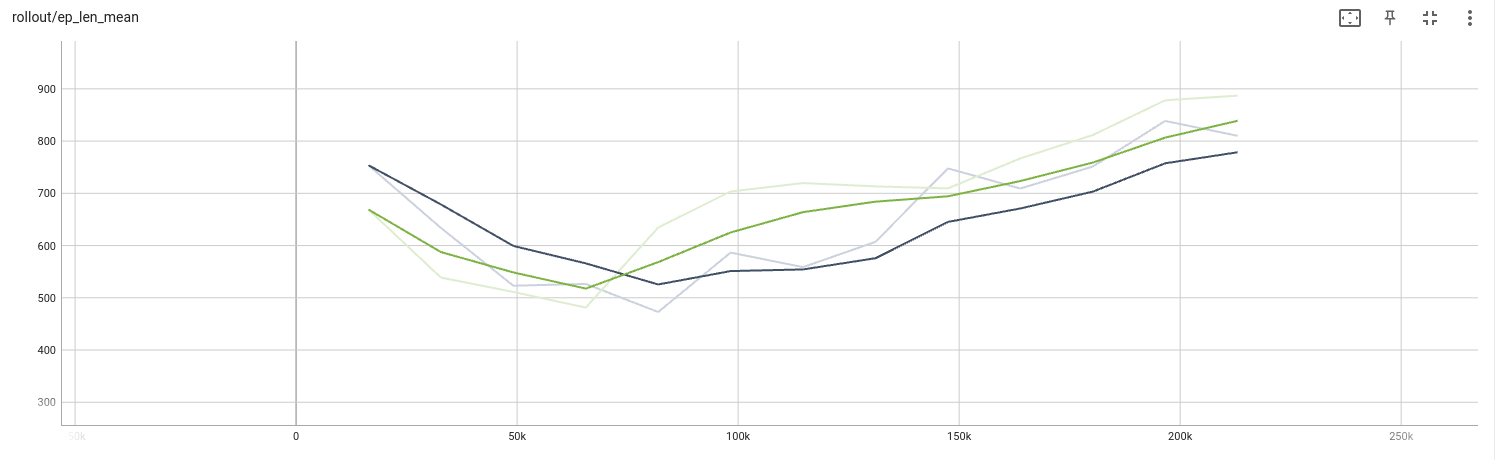
\includegraphics[width=1\linewidth]{Results/PPO_CNN/ep_length.png}
	\caption{ Episode Length}
	\label{f:g1}	
\end{figure}


\begin{figure}[ht]
	\centering
	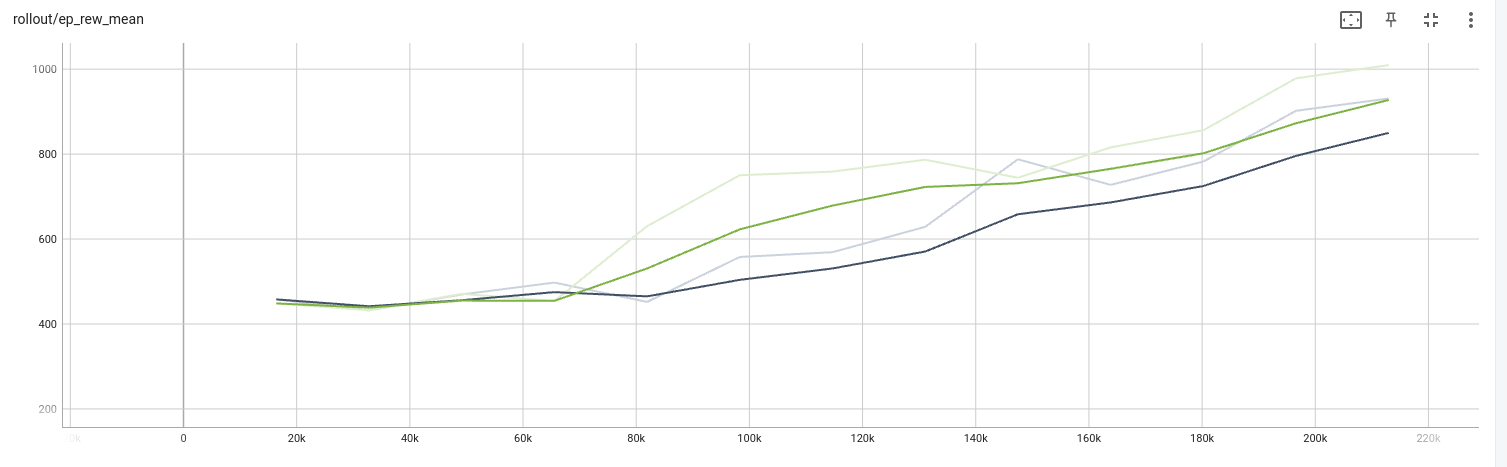
\includegraphics[width=1\linewidth]{Results/PPO_CNN/ep_reward.png}
	\caption{ Episode Reward }
	\label{f:g2}	
\end{figure}

\begin{figure}[ht]
	\centering
	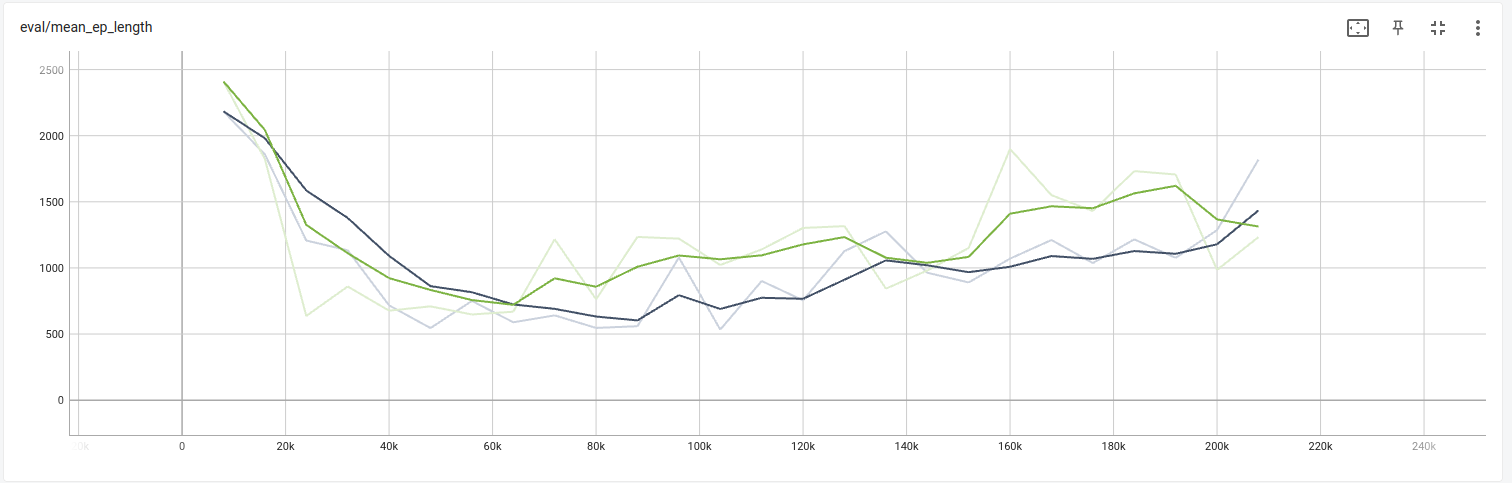
\includegraphics[width=1\linewidth]{Results/PPO_CNN/eval_length.png}
	\caption{ Evaluation Length}
	\label{f:g3}	
\end{figure}

\begin{figure}[ht]
	\centering
	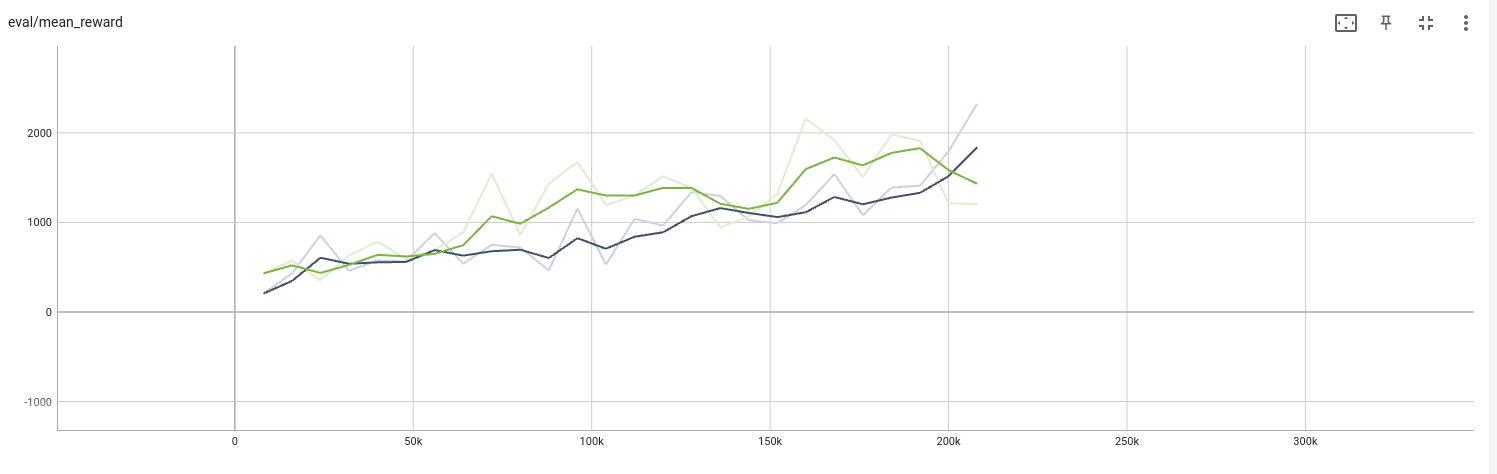
\includegraphics[width=1\linewidth]{Results/PPO_CNN/eval_reward.png}
	\caption{ Evaluation Reward}
	\label{f:g4}	
\end{figure}


\begin{figure}[ht]
	\centering
	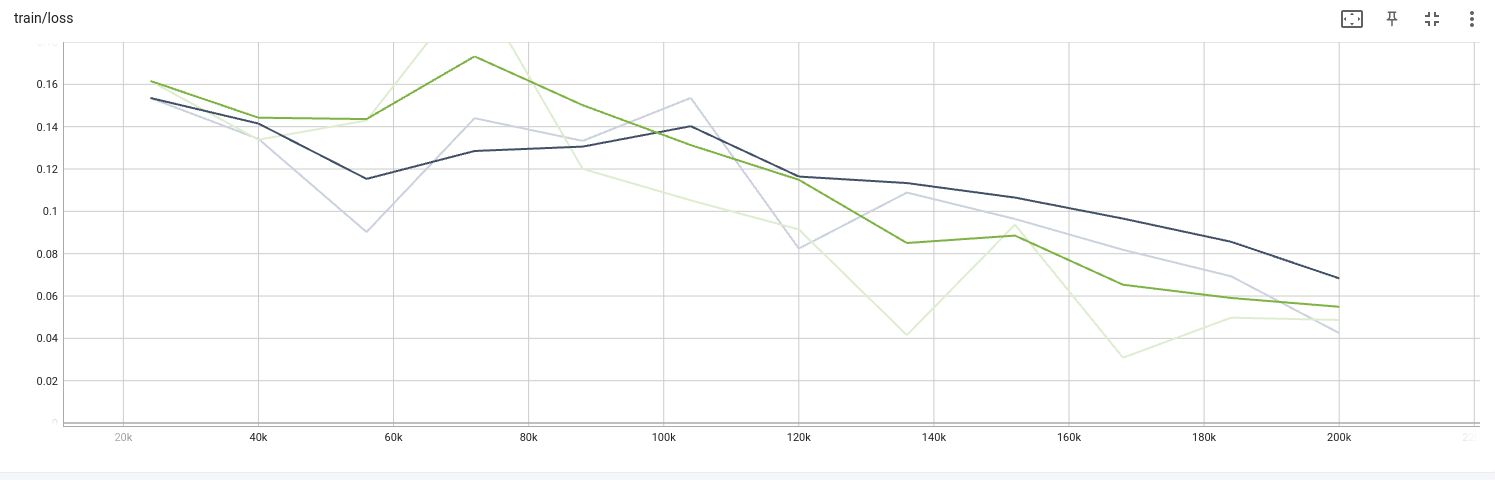
\includegraphics[width=1\linewidth]{Results/PPO_CNN/train_loss.png}
	\caption{Train loss}
	\label{f:g5}	
\end{figure}

\clearpage 


\subsection{Default MlpPolicy vs Custom MlpPolicy}

Στις δύο επόμενες εκπαιδεύσεις έχουν παραχθει τα παρακάτω 5 διαγράμματα \ref{f:g41}, \ref{f:g51}, \ref{f:g6}, \ref{f:g7} \ref{f:g8}, όπως και πιο πανω. Η μπλέ γραμμή αντιστοιχεί στο CustomMlpPolicy και η ροζ στο DefaultMlpPolicy. Στην συγκεκριμένη περίπτωση παρατηρούμε οτι 
το DefaultMlpPolicy παρόλο που έχει μεγαλύτερο reward και length στα τελευταία βήματα απο ότι το custom στο evalutation πέφτει πολύ πιο κάτω απο το episode. Αυτό οφείλεται σε overfitting(ίσως reverse exploration-exploitation trade-off) του default αφου η μεγιστη τιμή στο episode reward ειναι σχεδόν 800 ενώ στο evaluation οριακά φτάνει στο 500. Μεγαλύτερη διαφορά παρατηρείται αντίστοιχα μεταξυ episode length και evaluation length. Από την άλλη το custom στο evalutation ανεβαινει σχεδόν στο διπλασιο το reward του σε σχέση με το episode, τότε έχουμε exploration-exploitation-trade-off. Δηλαδή κατα την διάρκεια του training episode ο agent δοκιμάζει μόνο actions χωρίς να δίνει έμφαση στα policies που το βοηθάνε να σκοτώσει τους εχθρούς και να μαζέψει ποντους οπότε παιρνει χαμηλο reward και δεν διαρκεί πολυ το παιχνιδι. Απο την άλλη κατα την evaluation κατάσταση χρησιμοποιείται μόνο το exploitation των policies και έχει συνέχως μεγάλα rewards, κατι που παρατηρουμε και στα episode/reward lengths διαγράμματα \ref{f:g41}, \ref{f:g8}



\begin{figure}[ht]
	\centering
	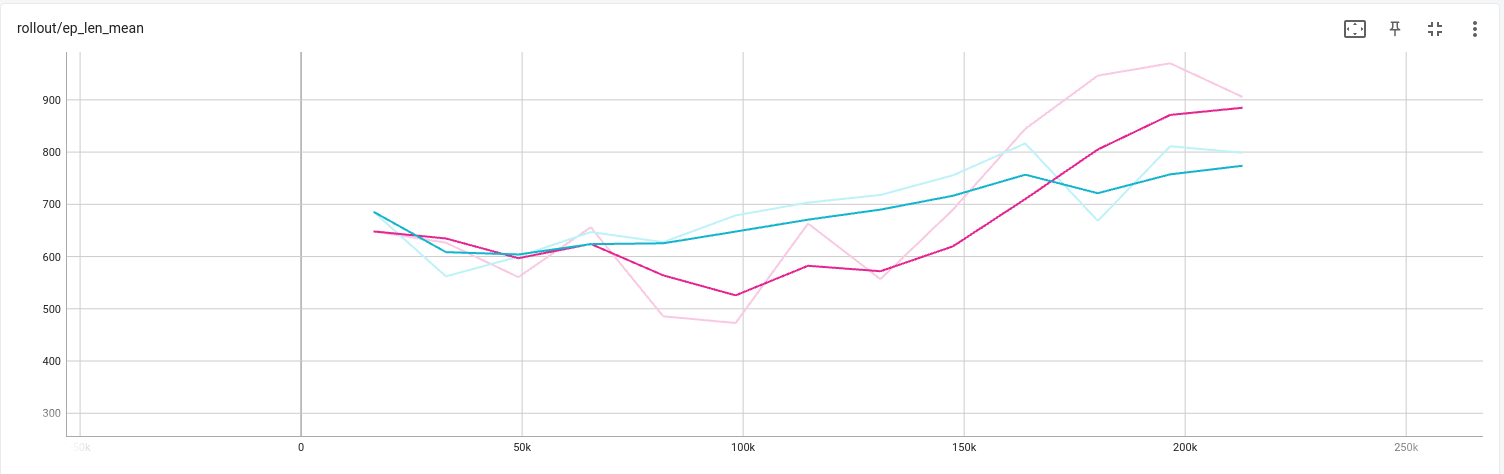
\includegraphics[width=1\linewidth]{Results/PPO_MLP/ep_length.png}
	\caption{ Episode Length}
	\label{f:g41}	
\end{figure}


\begin{figure}[ht]
	\centering
	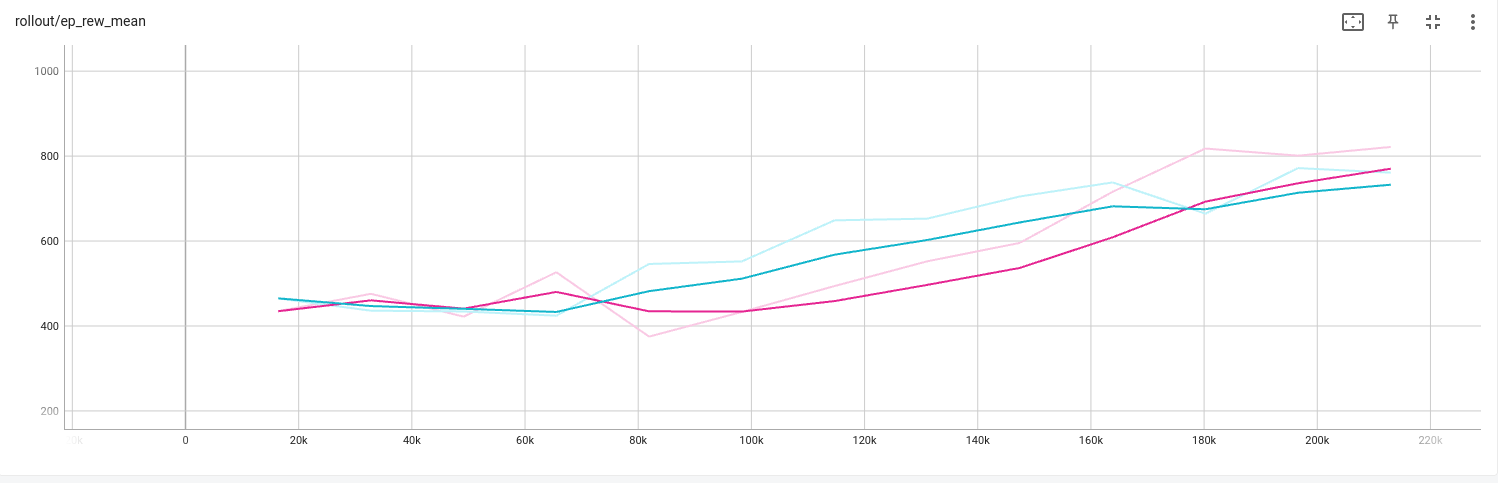
\includegraphics[width=1\linewidth]{Results/PPO_MLP/ep_reward.png}
	\caption{ Episode Reward }
	\label{f:g51}	
\end{figure}

\begin{figure}[ht]
	\centering
	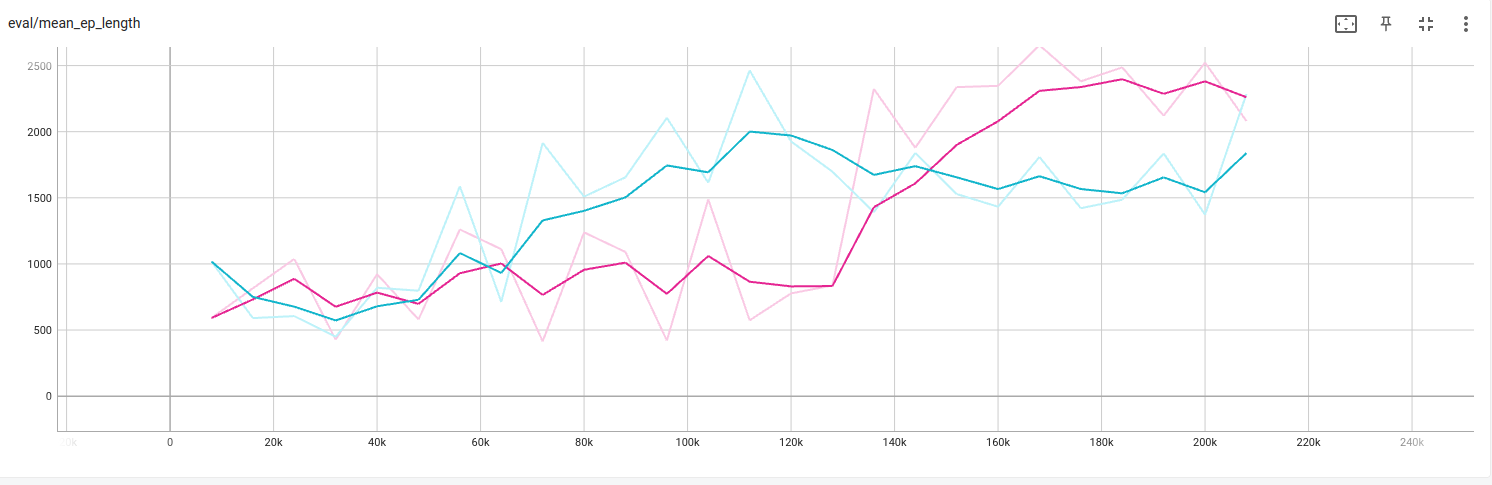
\includegraphics[width=1\linewidth]{Results/PPO_MLP/eval_length.png}
	\caption{ Evaluation Length}
	\label{f:g6}	
\end{figure}

\begin{figure}[ht]
	\centering
	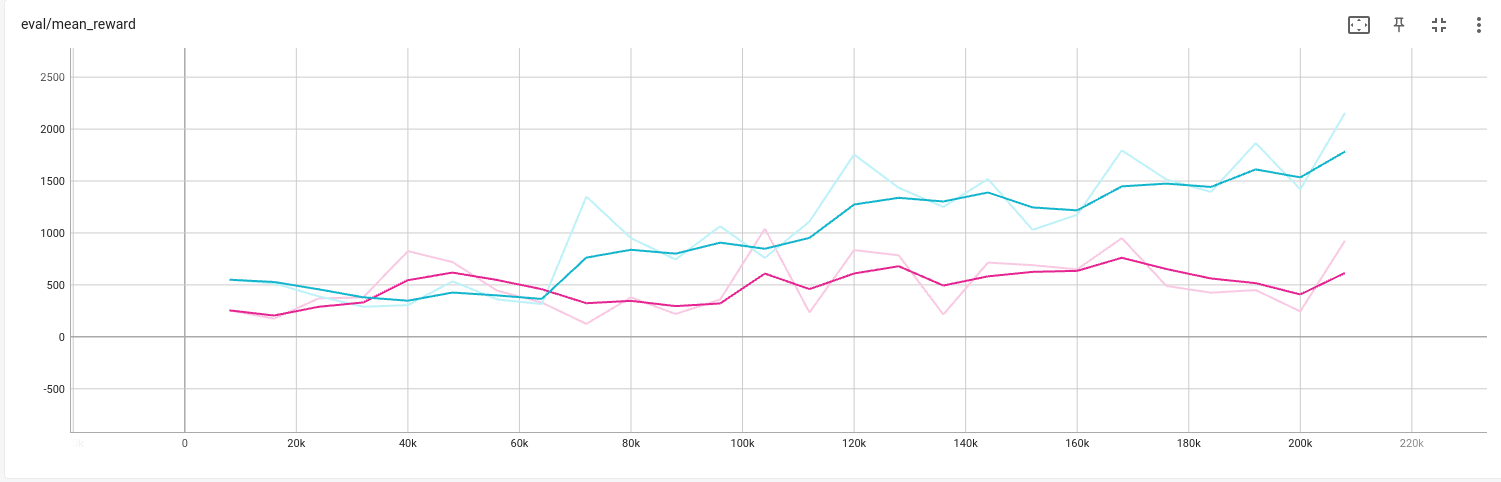
\includegraphics[width=1\linewidth]{Results/PPO_MLP/eval_reward.png}
	\caption{ Evaluation Reward}
	\label{f:g7}	
\end{figure}


\begin{figure}[ht]
	\centering
	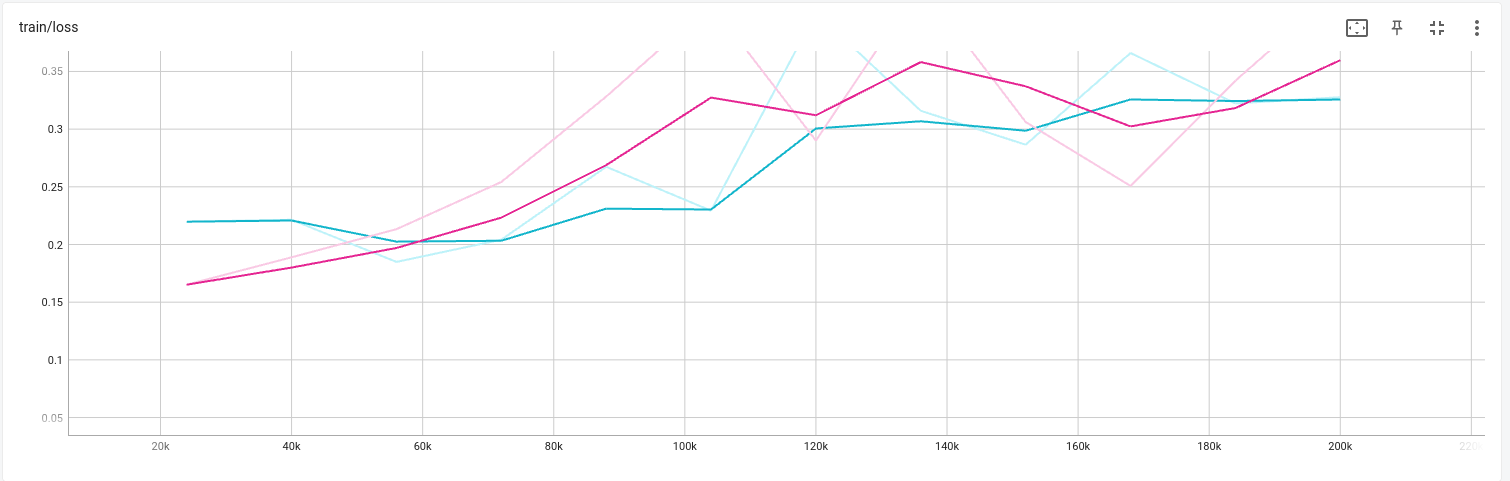
\includegraphics[width=1\linewidth]{Results/PPO_MLP/train_loss.png}
	\caption{Train loss}
	\label{f:g8}	
\end{figure}
\clearpage

\section{A2C Algorithm}
Με τον αλγόριθμο A2C έγιναν 4 εκαπιδέυσεις:

1. Η εκπαίδευση πραγματοποιήθηκε με CNNPolicy, xωρίς ορίσματα (defaultCNNPolicy).

2. Η εκπαίδευση πραγματοποιήθηκε με CNNPolicy και με όρισμα το CNN μοντέλο (customCNNPolicy).

3. Η εκπαίδευση πραγματοποιήθηκε με MlpPolicy χωρίς ορίσματα (defaultMlpPolicy) .

4. Η εκπαίδευση πραγματοποιήθηκε με MlpPolixy και με όρισμα το NN μοντέλο (customMlpPolicy).



\subsection{Default CNNPolicy vs Custom CNNPolicy}



Στις δύο πρωτες εκπαιδεύσεις έχουν παραχθεί τα παρακάτω 4 διαγράμματα \ref{f:g9}, \ref{f:g10}, \ref{f:g11}, \ref{f:g12}.
Η πορτοκαλί γραμμή αντιστοιχεί στο CustomCNNPolicy και η ροζ στο DefaultCNNPolicy. Παρατηρείται και εδώ στο DefaultCNNPolicy μοντέλο exploration-exploitation trade-off, αφού το evaluation reward ειναι 2000 ενώ το episode reward είναι κάτω απο 1000. Απο την άλλη ενώ το customCNNPolicy έχει χαμηλή απόδοση παραμένει παρόμοια και στα δύο περιβάλλοντα. Το episode length του σε κάποιες στιγμές φτάνει να είναι ίδιο με του Default που αυτο μας δίνει να καταλαβουμε οτι ο agent έχει μάθει να προσπαθεί στο ελάχιστο για να μην χάσει.






\begin{figure}[ht]
	\centering
	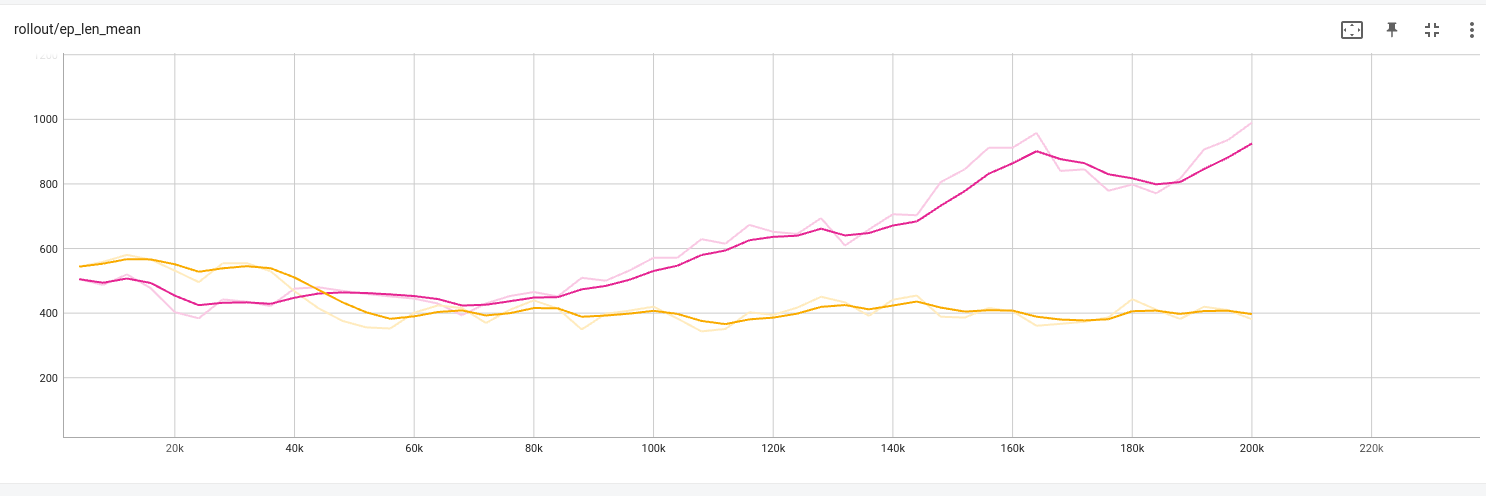
\includegraphics[width=1\linewidth]{Results/A2C_CNN/ep_length.png}
	\caption{ Episode Length}
	\label{f:g9}	
\end{figure}


\begin{figure}[ht]
	\centering
	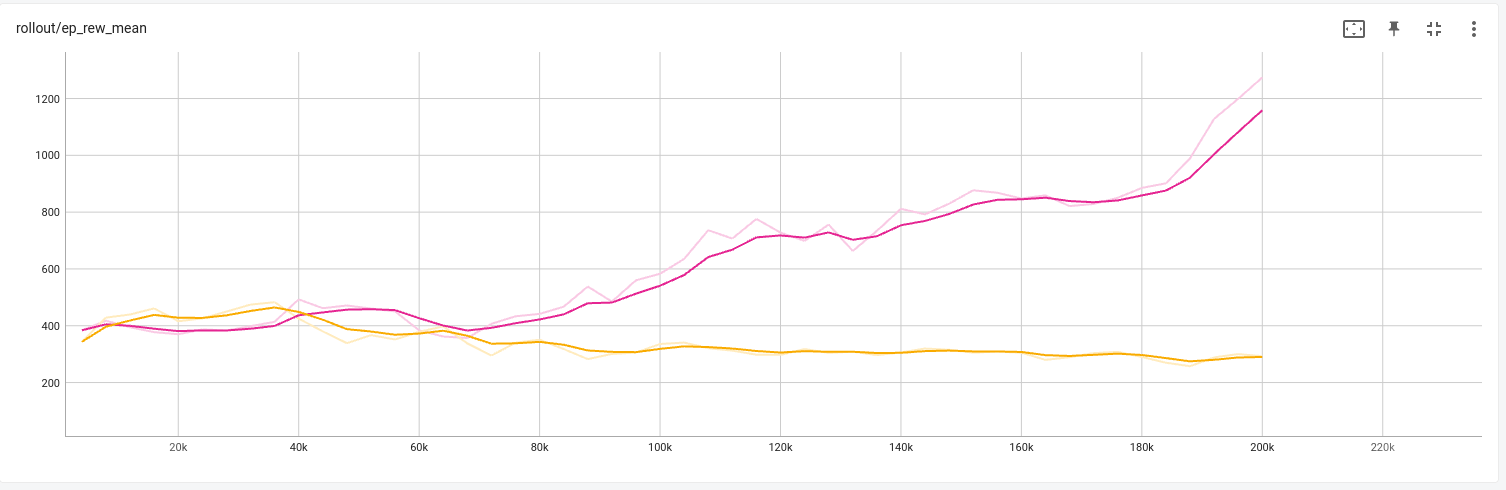
\includegraphics[width=1\linewidth]{Results/A2C_CNN/ep_reward.png}
	\caption{ Episode Reward }
	\label{f:g10}	
\end{figure}

\begin{figure}[ht]
	\centering
	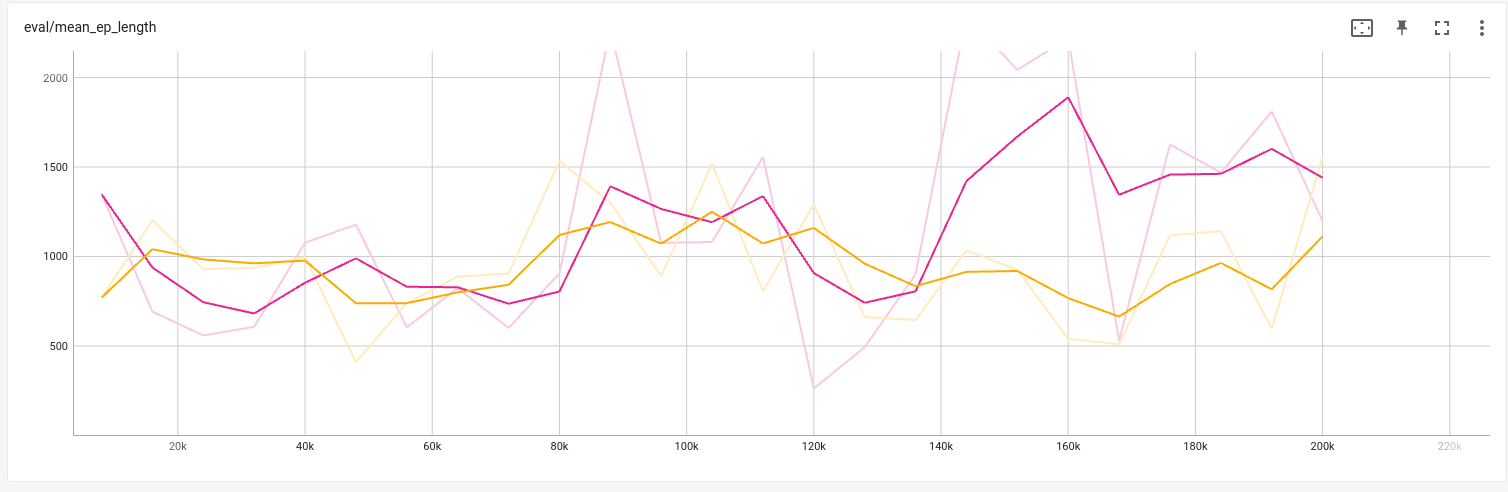
\includegraphics[width=1\linewidth]{Results/A2C_CNN/eval_length.png}
	\caption{ Evaluation Length}
	\label{f:g11}	
\end{figure}

\begin{figure}[ht]
	\centering
	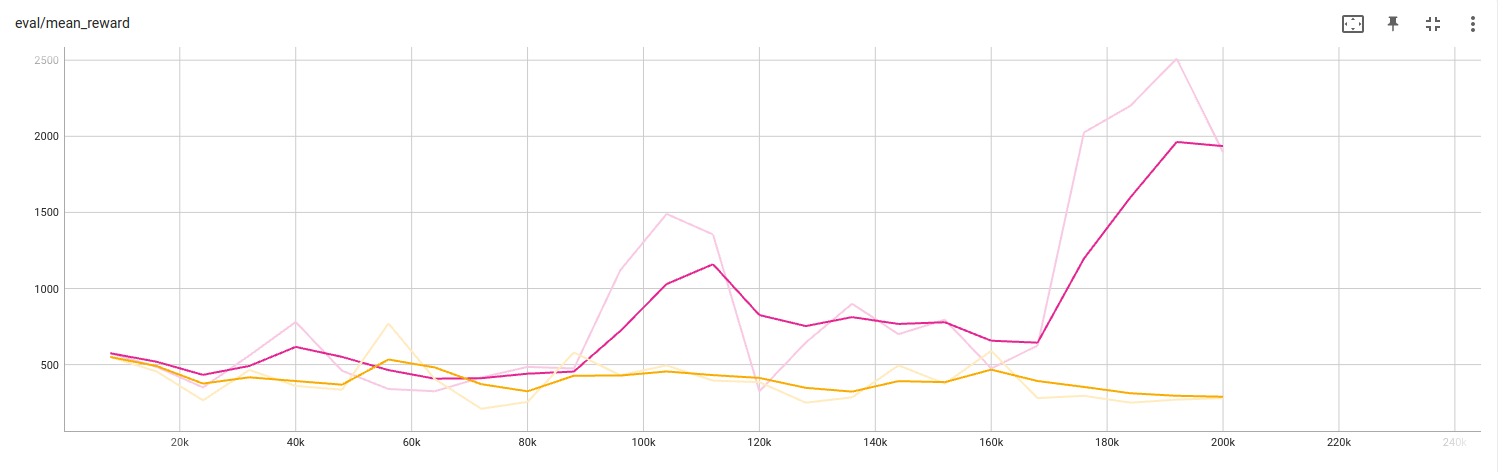
\includegraphics[width=1\linewidth]{Results/A2C_CNN/eval_reward.png}
	\caption{ Evaluation Reward}
	\label{f:g12}	
\end{figure}

\clearpage

\subsection{Default Mlpolicy vs Custom MlpPolicy}

Στις δύο επόμενες εκπαιδεύσεις έχουν παραχθεί τα παρακάτω 4 διαγράμματα \ref{f:g13}, \ref{f:g14}, \ref{f:g15}, \ref{f:g16}, όπως πιο πάνω.
Η μπλέ γραμμή αντιστοιχεί στο CustomMlp και η μάυρη αντιστοιχεί στο Default. Αυτό που παρατηρείται και στις δυο περιπτώσεις είναι οτι το length τόσο του evaluation όσο και του episode είναι παρα πολυ υψηλό σε σχεση με τα αντίστοιχα rewards. Αυτό μπορεί να οφείλεται
Exploration vs. Exploitation, Suboptimal Policy, Sparse Rewards :

Ο αλγόριθμος A2C εξισορροπεί το exploration (δοκιμή νέων ενεργειών) με το exploitation (επιλογή ενεργειών που είναι πιθανό να αποφέρουν υψηλές ανταμοιβές). Εάν το length είναι σταθερά υψηλότερο από το reward, αυτό μπορεί να υποδεικνύει ότι ο agent εξερευνά κυρίως το περιβάλλον και δεν εκμεταλλεύεται ακόμη τη βέλτιστη στρατηγική για τη μεγιστοποίηση των ανταμοιβών, και επειδή σταματάμε στα 200000 βήματα που είναι σχετικά μικρή τιμή για RL, δεν ξέρουμε αν μετά ανέβει το reward

Επίσης το customCNN μοντέλο που περνάει στο CNNPolicy ενδέχεται να μην μαθαίνει αποτελεσματικά τα υποκείμενα μοτίβα του παιχνιδιού. Η αρχιτεκτονική του μοντέλου, οι υπερπαράμετροι ή η διαδικασία εκπαίδευσης μπορεί να προκαλούν τo policy να παράγει ενέργειες που δεν ευθυγραμμίζονται με τη μεγιστοποίηση των rewards.

Τέλος τέτοιους είδους παιχνδίδια έχουν συνήθως sparse rewards signals, πράγμα που σημαίνει ότι ο agent λαμβάνει θετικά rewards σπάνια. Αυτό μπορεί να κάνει τη μάθηση πιο δύσκολη, καθώς ο agent μπορεί να δυσκολεύεται να συσχετίσει συγκεκριμένες ενέργειες με τις καθυστερημένα rewards. Σε τέτοιες περιπτώσεις, μπορεί να χρειαστεί περισσότερος χρόνος για να μάθει ο agent μια αποτελεσματική πολιτική που να επιτυγχάνει σταθερά υψηλά rewards.





\begin{figure}[ht]
	\centering
	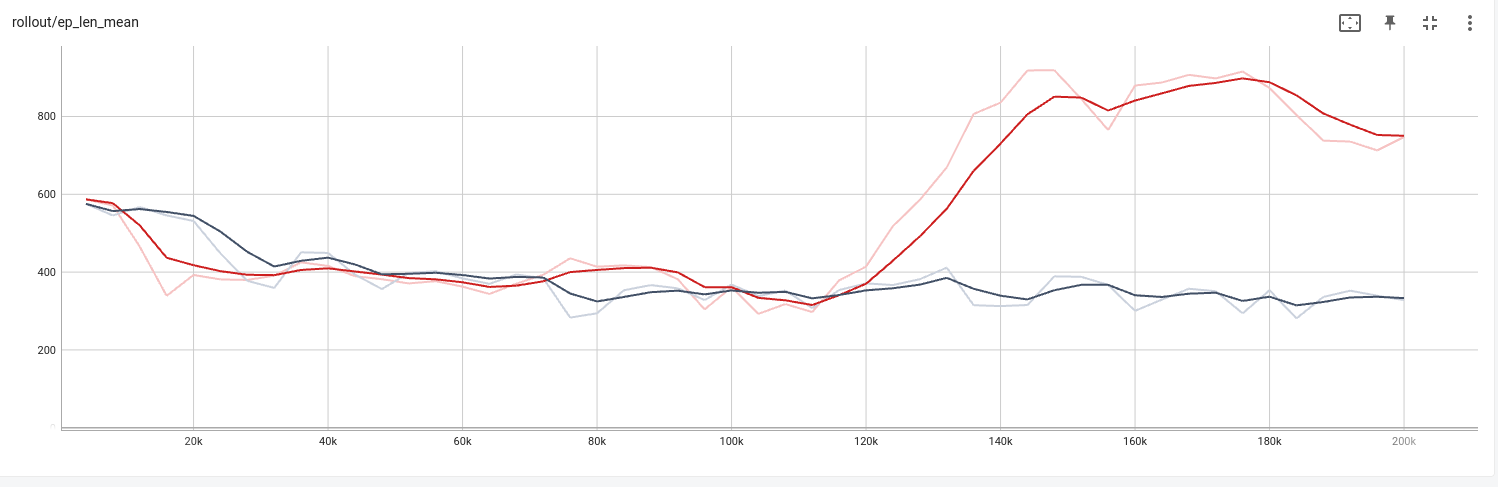
\includegraphics[width=1\linewidth]{Results/A2C_MLP/ep_length.png}
	\caption{ Episode Length}
	\label{f:g13}	
\end{figure}


\begin{figure}[ht]
	\centering
	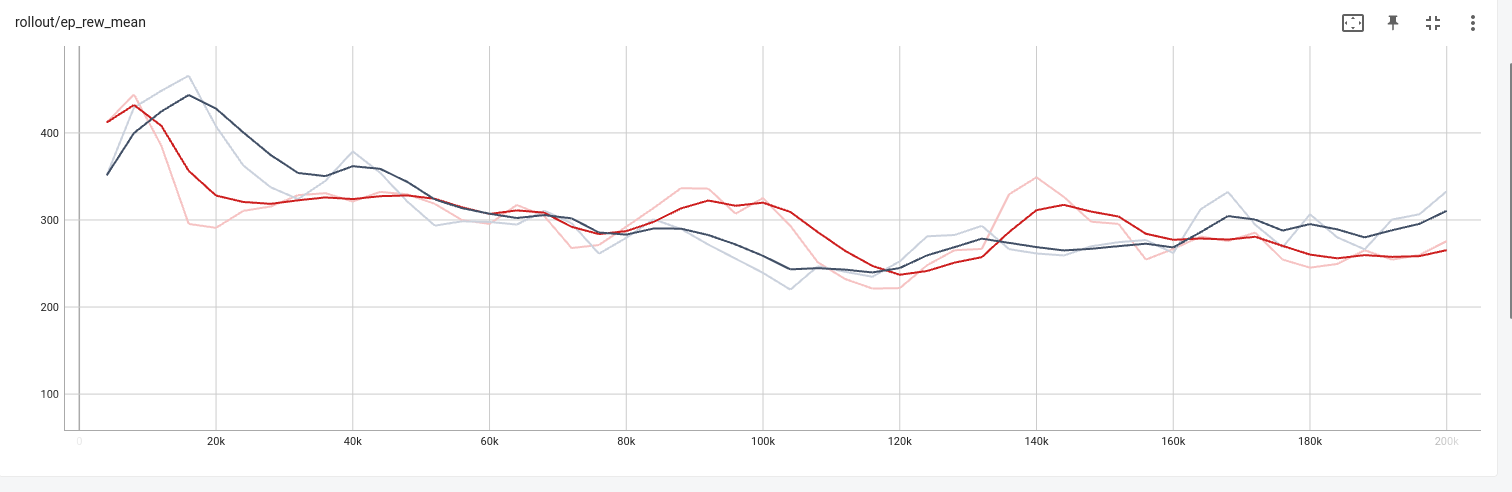
\includegraphics[width=1\linewidth]{Results/A2C_MLP/ep_reward.png}
	\caption{ Episode Reward }
	\label{f:g14}	
\end{figure}

\begin{figure}[ht]
	\centering
	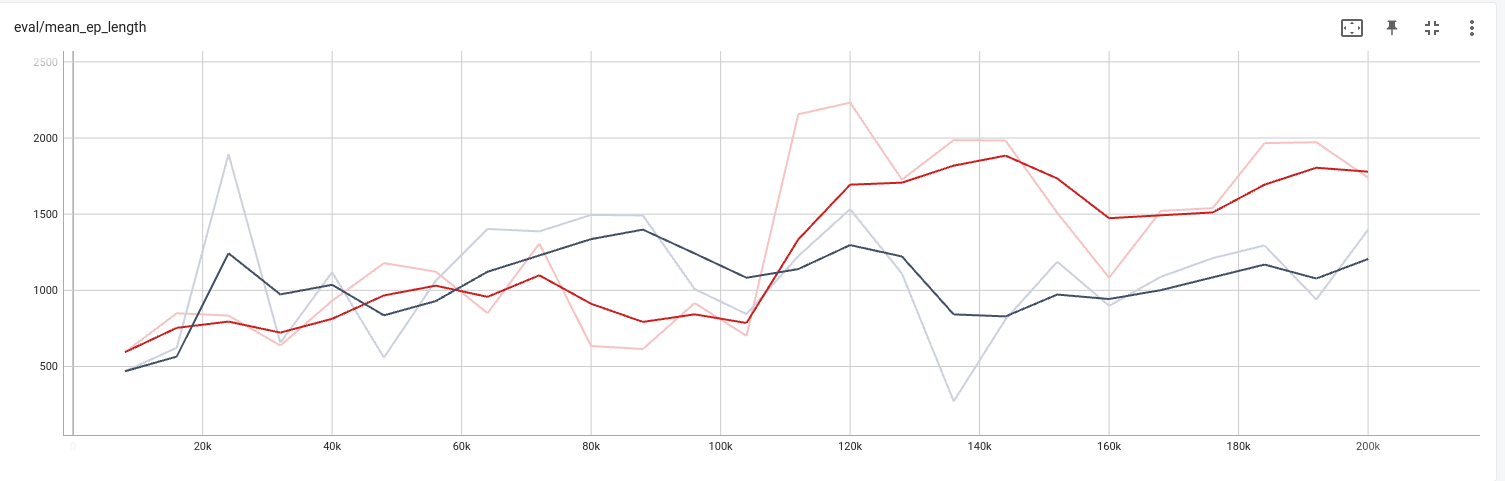
\includegraphics[width=1\linewidth]{Results/A2C_MLP/eval_length.png}
	\caption{ Evaluation Length}
	\label{f:g15}	
\end{figure}

\begin{figure}[ht]
	\centering
	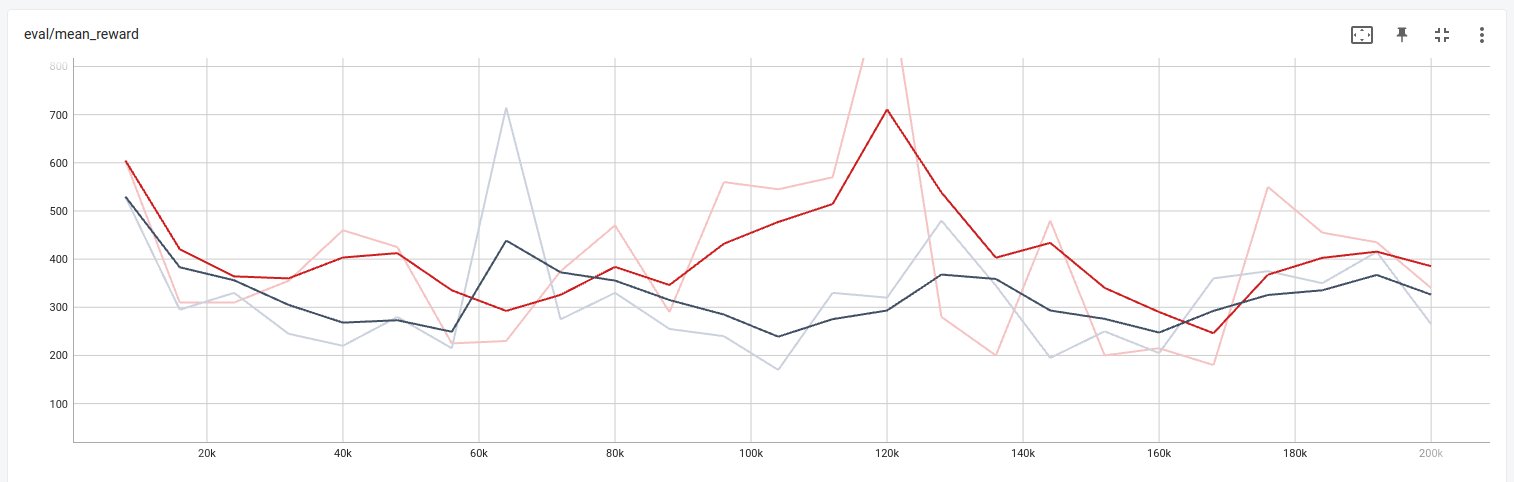
\includegraphics[width=1\linewidth]{Results/A2C_MLP/eval_reward.png}
	\caption{ Evaluation Reward}
	\label{f:g16}	
\end{figure}
\clearpage

\section{PPO vs A2C}

Στο τέλος συγκρίνουμε όλες τι εκπαιδεύσεις και παρατηρουμε στα δύο διαγράμμα \ref{f:g17}, \ref{f:g18}, ότι το A2C με defaultCNNPolicy έχει την καλύτερη απόδοση στο reward. Το PPO με customCNNPolicy στο episode reward διάγραμμα φαίνεται οτι έχει σταθερή αύξηση, ενώ στο evaluation reward διάγραμμα ξεκινάει στο τέλος να πέφτει. Τα δύο μοντέλα που έχουν σχετικά καλές αποδόσεις είναι τα PPO MLPCustomPolicy και PPO DefaultCnnPolicy, Τα υπόλοιπα μοντέλα είναι πιο ασταθή στην διάρκεια του χρόνου.

\begin{figure}[ht]
	\centering
	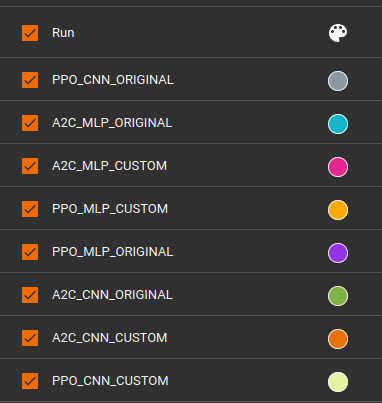
\includegraphics[width=0.4\linewidth]{Results/A2CvPPO/colors.png}
	\caption{ Color of the Models}
	\label{f:g19}	
\end{figure}

\begin{figure}[ht]
	\centering
	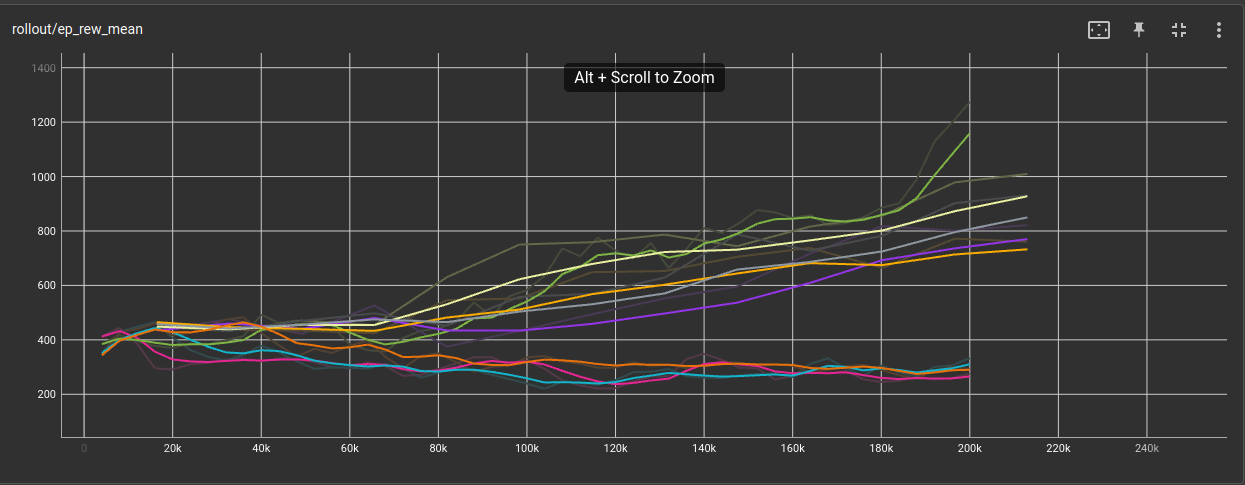
\includegraphics[width=1\linewidth]{Results/A2CvPPO/ep_reward.png}
	\caption{ Episode Reward }
	\label{f:g17}	
\end{figure}

\begin{figure}[ht]
	\centering
	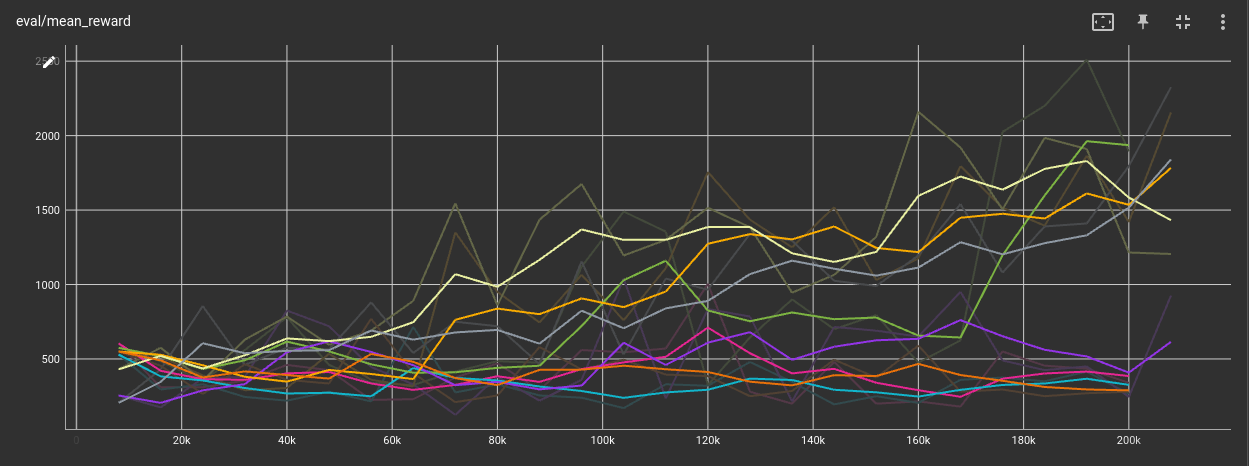
\includegraphics[width=1\linewidth]{Results/A2CvPPO/eval_reward.png}
	\caption{ Evaluation Reward}
	\label{f:g18}	
\end{figure}



	%\appendix
	%\chapter{Code}
	%\label{appendix:app}
	%\section{Code CNN-numpy}

\begin{lstlisting}[language=Python, caption=Convolutional Layer]
	
	import numpy as np
	from scipy import signal
	
	class Convolution_Layer(Layer):
	def __init__(self, input_shape, kernel_size, depth):
	input_depth, input_height, input_width = input_shape
	self.depth = depth
	self.input_shape = input_shape
	self.input_depth = input_depth
	self.output_shape = (depth, input_height - kernel_size + 1, input_width - kernel_size + 1)
	self.kernels_shape = (depth, input_depth, kernel_size, kernel_size) # Το depth μας δίνει τον αριθμο των kernels, Το input depth τις διαστασεις του input, και το kernel size μας δινει το μεγεθος του πινακα στους kernel
	self.kernels = np.random.randn(*self.kernels_shape)                # Για παραδειγμα αν εχω ενα τρισδιαστατο input(3 καναλια), και εχω βαλει depth 5, και kernel sizei 3*3, θα εχω(5,3,3,3) 
	self.biases = np.random.randn(*self.output_shape)
	
	def forward(self, input):
	self.input = input
	self.output = np.copy(self.biases)
	for i in range(self.depth):
	for j in range(self.input_depth):
	self.output[i] += signal.correlate2d((self.input[j]), (self.kernels[i, j]), "valid")
	return self.output
	
	def backwards(self, d_output):
	self.d_kernels = np.zeros(self.kernels_shape)
	self.d_inputs= np.zeros(self.input_shape)
	
	for i in range(self.depth):
	for j in range(self.input_depth):
	self.d_kernels[i, j] = signal.correlate2d(self.input[j], d_output[i], "valid")
	self.d_inputs[j] += signal.convolve2d(d_output[i], self.kernels[i, j], "full")
	self.d_biases = np.sum(d_output,axis=0,keepdims=True)  
	
	class Layer:
	def __init__(self):
	self.input = None
	self.output = None
	
	def forward(self, input):
	# TODO: return output
	pass
	
	def backward(self, output_gradient):
	# TODO: update parameters and return input gradient
	pass
	
\end{lstlisting}


\begin{lstlisting}[language=Python, caption=Dense Layer]
	class Layer_Dense:
	#Initialization of Layers
	def __init__(self,n_inputs,n_neurons):
	self.weights = 0.01* np.random.randn(n_inputs, n_neurons) 
	self.biases = np.zeros((1,n_neurons))
	
	#Forward pass
	def forward(self,inputs):
	self.inputs = inputs
	self.output = np.dot(inputs,self.weights) + self.biases
	
	def backwards(self, d_output):
	self.d_weights = np.dot(self.inputs.T,d_output)
	
	self.d_biases = np.sum(d_output,axis=0,keepdims=True)   
	
	self.d_inputs = np.dot(d_output,self.weights.T)
	
\end{lstlisting}


\begin{lstlisting}[language=Python, caption=ReLU Layer]
	class Activation_ReLU:
	def forward(self,inputs):
	self.inputs = inputs
	self.output = np.maximum(0,inputs)
	
	def backwards(self, d_output):
	self.d_inputs = d_output.copy()
	
	self.d_inputs[self.inputs<=0] = 0
	
\end{lstlisting}


\begin{lstlisting}[language=Python, caption=Reshape Layer]
	class Reshape(Layer):
	def __init__(self, input_shape, output_shape):
	self.input_shape = input_shape
	self.output_shape = output_shape
	
	def forward(self, input):
	self.output = np.reshape(input, self.output_shape)
	self.output= self.output.T
	
	def backwards(self, output_gradient):
	self.d_inputs = np.reshape(output_gradient, self.input_shape)
	
		class Layer:
	def __init__(self):
	self.input = None
	self.output = None
	
	def forward(self, input):
	# TODO: return output
	pass
	
	def backward(self, output_gradient):
	# TODO: update parameters and return input gradient
	pass
	
\end{lstlisting}

\begin{lstlisting}[language=Python, caption=Dropout Layer]
	import numpy as np
	
	class Dropout_Layer:
	
	def __init__(self, rate):
	self.rate = 1 -rate
	
	def forward(self, inputs):
	
	self.inputs = inputs
	
	
	self.binary_mask = np.random.binomial(1,self.rate,size=inputs.shape) / self.rate
	
	self.output = inputs * self.binary_mask
	
	def backwards(self, d_output):
	
	self.d_inputs = d_output * self.binary_mask
	
\end{lstlisting}

\begin{lstlisting}[language=Python, caption=Softmax Activation]
	import numpy as np
	
	
	class Activation_Softmax:
	
	def __init__(self):
	self.predictions = []
	def forward(self,inputs):
	self.inputs = inputs
	
	exp_values = np.exp(inputs-np.max(inputs, axis=1, keepdims=True))
	probabilities = exp_values / np.sum(exp_values, axis=1, keepdims=True)
	self.output = probabilities
	self.predictions.append(probabilities)
	# print(predictions)
	
	
	def backwards(self,d_output):
	self.d_inputs = np.empty_like(d_output)
	
	for index, (single_output,single_d_output) in enumerate(zip(self.output,d_output)):
	single_output = single_output.reshape(-1,1)
	
	jacobian_matrix = np.diagflat(single_output) - np.dot(single_output,single_output.T)
	
	self.d_inputs[index] = np.dot(jacobian_matrix,single_d_output)
	
	
	def predictions(self,output):
	# print(np.argmax(output,axis=1))
	return np.argmax(output,axis=1)

\end{lstlisting}

\begin{lstlisting}[language=Python, caption=Loss function]
	import numpy as np
	
	class Loss:
	def remember_trainable_layers(self,trainable_layers):
	self.trainable_layers = trainable_layers
	
	def calculate(self,output,y):
	sample_losses= self.forward(output,y)
	
	data_loss = np.mean(sample_losses)
	
	
	return data_loss
	
	class Loss_CategoricalCrossentropy(Loss):
	def forward(self,y_pred,y_true):
	samples = len(y_pred)
	y_pred_clipped = np.clip(y_pred, 10e-3, 1.0 - 10e-3)
	
)
	if len(y_true.shape) == 1:
	correct_confidences = y_pred_clipped [range(samples), y_true.T]
	
	elif len(y_true.shape) == 2:
	correct_confidences = np.sum(y_pred_clipped*y_true,axis=1)
	negative_log_likelihood = -np.log(correct_confidences)
	return negative_log_likelihood
	
	def backwards(self,d_output,y_true):
	samples =len(d_output)
	labels = len(d_output[0])
	if len(y_true.shape) == 1:
	print('yehaw')
	y_true = np.eye(labels)[y_true]
	
	self.d_inputs = -y_true.T/d_output
	self.d_inputs = self.d_inputs /samples
	

\end{lstlisting}

\begin{lstlisting}[language=Python, caption=Optimizer function]
	import numpy as np 
	from Conv_layer import *
	from Dense_layer import *
	
	class Optimizer_SGD:
	
	def __init__(self, learning_rate=0.01, decay=0, momentum=0):
	self.learning_rate = learning_rate
	self.current_learning_rate = learning_rate
	self.decay = decay
	self.iterations = 0
	self.momentum = momentum
	
	def pre_update_parameters(self):
	if self.decay:
	self.current_learning_rate = self.learning_rate * (1. / (1. + self.decay * self.iterations))
	
	def update_parameters(self, layer):
	if isinstance(layer, Convolution_Layer):
	if self.momentum:
	
	if not hasattr(layer, 'kernel_momentums'):
	
	layer.kernel_momentums = np.zeros_like(layer.kernels)
	layer.bias_momentums = np.zeros_like(layer.biases)
	
	kernel_updates = self.momentum * layer.kernel_momentums - self.current_learning_rate * layer.d_kernels
	layer.kernel_momentums = kernel_updates
	
	bias_updates = self.momentum * layer.bias_momentums - self.current_learning_rate * layer.d_biases
	layer.bias_momentums = bias_updates
	
	else :
	kernel_updates= -self.current_learning_rate * layer.d_kernels
	bias_updates = -self.current_learning_rate * layer.d_biases
	
	layer.kernels += kernel_updates
	layer.biases += bias_updates
	
	elif isinstance(layer, Layer_Dense):
	if self.momentum:
	
	if not hasattr(layer, 'weight_momentums'):
	layer.weight_momentums = np.zeros_like(layer.weights)
	layer.bias_momentums = np.zeros_like(layer.biases)
	
	weight_updates = self.momentum * layer.weight_momentums - self.current_learning_rate * layer.d_weights
	layer.weight_momentums = weight_updates
	
	bias_updates = self.momentum * layer.bias_momentums - self.current_learning_rate * layer.d_biases
	layer.bias_momentums = bias_updates
	
	else :
	weight_updates= -self.current_learning_rate * layer.d_weights
	bias_updates = -self.current_learning_rate * layer.d_biases
	layer.weights += weight_updates
	layer.biases += bias_updates
	
	def post_update_parameters(self):
	self.iterations += 1
	
	
	
	
	
	
	class Optimizer_Adam:
	
	def __init__(self, learning_rate=10e-4, decay = 0, epsilon = 1e-7, beta1=0.9, beta2=0.999):
	self.learning_rate = learning_rate
	self.current_learning_rate = learning_rate
	self.decay = decay
	self.iterations = 0
	self.epsilon = epsilon
	self.beta1 = beta1
	self.beta2 = beta2
	
	def pre_update_parameters(self):
	if self.decay:
	self.current_learning_rate = self.learning_rate * (1. /(1. + self.decay * self.iterations))
	
	
	def update_parameters(self, layer):
	if isinstance(layer, Convolution_Layer):
	if not hasattr(layer, 'kernels_cache'):
	layer.bias_cache = np.zeros_like(layer.biases)
	layer.bias_momentums = np.zeros_like(layer.biases)
	layer.kernels_cache = np.zeros_like(layer.kernels)
	layer.kernels_momentums = np.zeros_like(layer.kernels)
	
	layer.bias_momentums = self.beta1 * layer.bias_momentums + (1 - self.beta1) * layer.d_biases
	layer.kernels_momentums = self.beta1 * layer.kernels_momentums + (1 - self.beta1) * layer.d_kernels
	
	bias_momentums_corrected = layer.bias_momentums / (1 - self.beta1 ** (self.iterations +1))
	kernels_momentums_corrected = layer.kernels_momentums / (1 - self.beta1 ** (self.iterations +1))
	
	layer.bias_cache = self.beta2 * layer.bias_cache + (1 - self.beta2) * layer.d_biases**2
	layer.kernels_cache = self.beta2 * layer.kernels_cache + (1 - self.beta2) * layer.d_kernels**2
	
	bias_cache_corrected = layer.bias_cache / (1 - self.beta2 ** (self.iterations+1))
	kernels_cache_corrected = layer.kernels_cache / (1 - self.beta2 ** (self.iterations+1))
	
	layer.biases += -self.current_learning_rate * bias_momentums_corrected / (np.sqrt(bias_cache_corrected) + self.epsilon)
	layer.kernels += -self.current_learning_rate * kernels_momentums_corrected / (np.sqrt(kernels_cache_corrected) + self.epsilon)
	
	
	elif isinstance(layer, Layer_Dense):
	if not hasattr(layer, 'weight_cache'):
	layer.weight_cache = np.zeros_like(layer.weights)
	layer.weight_momentums = np.zeros_like(layer.weights)
	layer.bias_cache = np.zeros_like(layer.biases)
	layer.bias_momentums = np.zeros_like(layer.biases)
	
	layer.weight_momentums = self.beta1 * layer.weight_momentums + (1 - self.beta1) * layer.d_weights
	layer.bias_momentums = self.beta1 * layer.bias_momentums + (1 - self.beta1) * layer.d_biases
	# print(layer.weight_momentums)
	weight_momentums_corrected = layer.weight_momentums / (1 - self.beta1 ** (self.iterations +1))
	bias_momentums_corrected = layer.bias_momentums / (1 - self.beta1 ** (self.iterations +1))
	
	layer.weight_cache = self.beta2 * layer.weight_cache + (1 - self.beta2) * layer.d_weights**2
	layer.bias_cache = self.beta2 * layer.bias_cache + (1 - self.beta2) * layer.d_biases**2
	
	
	weight_cache_corrected = layer.weight_cache / (1 - self.beta2 ** (self.iterations+1))
	bias_cache_corrected = layer.bias_cache / (1 - self.beta2 ** (self.iterations+1))
	
	layer.weights += -self.current_learning_rate * weight_momentums_corrected / (np.sqrt(weight_cache_corrected) + self.epsilon)
	layer.biases += -self.current_learning_rate * bias_momentums_corrected / (np.sqrt(bias_cache_corrected) + self.epsilon)
	# print(layer.weights)
	def post_update_parameters(self):
	self.iterations +=1

\end{lstlisting}	

\begin{lstlisting}[language=Python, caption=Model]
	import numpy as np
	from Conv_layer import *
	from Softmax_function import *
	from Loss_function import *
	from Dropout_layer import *
	from Dense_layer import *
	from Optimizer_function import *
	import tensorflow as tf
	from keras.datasets import mnist
	from keras.utils import np_utils
	import matplotlib.pyplot as plt
	from tqdm import tqdm
	import time as time
	
	
	plot_filename = "plot.png"
	model_output = "model.txt"
	
	# Preprocess Function
	data_limit = 100
	def preprocess_data(x, y):
	x_new = []
	y_new = []
	for i in range(10):
	indices = np.where(y == i)[0][:data_limit]
	np.random.shuffle(indices)  # Shuffle the indices before selecting data
	x_new.append(x[indices])
	y_new.append(np.full(len(indices), i))
	x_new = np.concatenate(x_new)
	y_new = np.concatenate(y_new)
	x_new = x_new.reshape(len(x_new), 1, 28, 28)
	x_new = x_new.astype("float32") / 255
	y_new = np_utils.to_categorical(y_new)
	y_new = y_new.reshape(len(y_new), 10, 1)
	indices = np.random.permutation(len(x_new))  # Shuffle the data
	return x_new[indices], y_new[indices]
	
	
	# Load mnist and preprocess data
	(x_train, y_train), (x_test, y_test) = mnist.load_data()
	X_train, y_train = preprocess_data(x_train, y_train)
	X_test, y_test = preprocess_data(x_test, y_test)
	
	# Initalize layers and functions
	dropout_dense_1 = Dropout_Layer(0.5)
	dropout_dense_2 = Dropout_Layer(0.2)
	conv_1 = Convolution_Layer((1, 28, 28), 3, 10)
	flatten=Reshape((10, 26, 26), (10 * 26 * 26, 1))
	dense_1 = Layer_Dense(10 * 26* 26,128)
	dense_2=Layer_Dense(128,10)
	activation_conv_1 = Activation_ReLU()
	activation_dense_1 = Activation_ReLU()
	activation_dense_2 = Activation_ReLU()
	softmax = Activation_Softmax()
	
	loss_function = Loss_CategoricalCrossentropy()
	# optimizer = Optimizer_Adam(learning_rate=10e-5,decay=10e-6)
	optimizer = Optimizer_SGD(learning_rate=10e-5,decay=0)
	
	train_losses = []
	train_accuracies = []
	test_losses = []
	test_accuracies = []
	
	
	
	
	with open(model_output, "w") as f:
	for epoch in tqdm(range(41)):
	softmax.predictions=[]
	start_time = time.time()
	for x, y in tqdm(zip(X_train, y_train), desc=f'Epoch {epoch}'):
	
	# Forward pass
	conv_1.forward(x)
	activation_conv_1.forward(conv_1.output)
	flatten.forward(activation_conv_1.output)
	dense_1.forward(flatten.output)
	activation_dense_1.forward(dense_1.output)
	dropout_dense_1.forward(activation_dense_1.output)
	dense_2.forward(dropout_dense_1.output)
	activation_dense_2.forward(dense_2.output)
	dropout_dense_2.forward(activation_dense_2.output)
	softmax.forward(dropout_dense_2.output)
	loss_function.forward(softmax.output, y)
	
	# Backward pass
	loss_function.backwards(softmax.output, y)
	softmax.backwards(loss_function.d_inputs)
	dropout_dense_2.backwards(softmax.d_inputs)
	activation_dense_2.backwards(dropout_dense_2.d_inputs)
	dense_2.backwards(activation_dense_2.d_inputs)
	dropout_dense_1.backwards(dense_2.d_inputs)
	activation_dense_1.backwards(dropout_dense_1.d_inputs)
	dense_1.backwards(activation_dense_1.d_inputs)
	flatten.backwards(dense_1.d_inputs)
	activation_conv_1.backwards(flatten.d_inputs)
	conv_1.backwards(activation_conv_1.d_inputs)
	
	# Optimize gradients
	optimizer.pre_update_parameters()
	optimizer.update_parameters(conv_1)
	optimizer.update_parameters(dense_1)
	optimizer.update_parameters(dense_2)
	optimizer.post_update_parameters()
	
	# Training accuracy calculation
	y_reshaped = y_train.reshape(data_limit*10,10)
	predictions_array =np.asarray(softmax.predictions)
	predictions_reshaped = predictions_array.reshape(y_reshaped.shape)
	predictions_reshaped_true= np.argmax(predictions_reshaped,axis=1)
	if len(y_reshaped.shape) == 2:
	train_labels=np.argmax(y_reshaped,axis=1)  
	train_predictions = predictions_reshaped_true.reshape(train_labels.shape)
	training_accuracy = np.mean(train_predictions==train_labels)
	train_accuracies.append(training_accuracy)
	train_accuracies.append(training_accuracy)
	
	#Training loss calculation
	loss = loss_function.calculate(predictions_reshaped, y_reshaped)
	train_losses.append(loss)
	
	
	# Test predictions
	softmax.predictions = []
	test_losses_epoch = []
	test_predictions = []
	for x, y in zip(X_test, y_test):
	
	# Forward pass
	conv_1.forward(x)
	activation_conv_1.forward(conv_1.output)
	flatten.forward(activation_conv_1.output)
	dense_1.forward(flatten.output)
	activation_dense_1.forward(dense_1.output)
	dropout_dense_1.forward(activation_dense_1.output)
	dense_2.forward(dropout_dense_1.output)
	activation_dense_2.forward(dense_2.output)
	dropout_dense_2.forward(activation_dense_2.output)
	softmax.forward(dropout_dense_2.output)
	loss_function.forward(softmax.output, y)
	
	
	# Calculate test accuracy and loss
	test_predictions = np.asarray(softmax.predictions)
	test_predictions = test_predictions.reshape(len(test_predictions), -1)
	test_labels = y_test.reshape(len(y_test), -1)
	test_loss = loss_function.calculate(test_predictions, test_labels)
	test_accuracy = np.mean(np.argmax(test_predictions, axis=1) == np.argmax(test_labels, axis=1))
	test_losses_epoch.append(test_loss)
	test_losses.append(np.mean(test_losses_epoch))
	test_accuracies.append(test_accuracy)
	
	if not epoch % 10:
	end_time = time.time()
	elapsed_time = end_time - start_time
	output = (f"Epoch {epoch} took {elapsed_time:.2f} seconds, "
	f"training loss: {loss:.3f}, "
	f"training accuracy: {training_accuracy:.3f}, "
	f"test loss: {test_loss:.3f}, "
	f"test accuracy: {test_accuracy:.3f}, "
	f"optimizer: {optimizer.current_learning_rate}\n")
	print(output, end="")
	
	f.write(output)
	
	
	
	# Plot training and test loss and accuracy
	def save_plot(filename,train_losses,test_losses,train_accuracies,test_accuracies):
	plt.figure(figsize=(10, 5))
	plt.subplot(1, 2, 1)
	plt.plot(train_losses, label='Training')
	plt.plot(test_losses, label='Test')
	plt.title('Loss')
	plt.xlabel('Epoch')
	plt.legend()
	
	plt.subplot(1, 2, 2)
	plt.plot(train_accuracies, label='Training')
	plt.plot(test_accuracies, label='Test')
	plt.title('Accuracy');
	plt.xlabel('Epoch')
	plt.legend()
	plt.savefig(filename)
	plt.show()
	
	save_plot(plot_filename,train_losses, test_losses,train_accuracies,test_accuracies)
	
\end{lstlisting}	

\section{Tensorflow-CNN}

\begin{lstlisting}[language=Python, caption=CNN]
	import tensorflow as tf
	from tensorflow.keras.models import Sequential
	from tensorflow.keras.layers import Conv2D, MaxPooling2D, Flatten, Dense, Dropout
	from tensorflow.keras.optimizers import SGD
	import numpy as np
	from tensorflow.keras.utils import to_categorical
	from tensorflow.keras.datasets import mnist
	import matplotlib.pyplot as plt
	# Set data limits and filenames
	import os
	
	# Define the path to the directory where the model will be saved
	model_dir = 'saved_models'
	os.makedirs(model_dir, exist_ok=True)
	
	# Save the model inside the directory
	
	data_limit = 4000
	plot_filename = "tensorflow_lr_moment_decay.png"
	# model_output = "model.txt"
	
	# Define a function to preprocess the data
	def preprocess_data(x, y):
	x_new = []
	y_new = []
	for i in range(10):
	indices = np.where(y == i)[0][:data_limit]
	np.random.shuffle(indices)  # Shuffle the indices before selecting data
	x_new.append(x[indices])
	y_new.append(np.full(len(indices), i))
	x_new = np.concatenate(x_new)
	y_new = np.concatenate(y_new)
	x_new = x_new.reshape(len(x_new), 28, 28, 1)
	x_new = x_new.astype("float32") / 255
	y_new = to_categorical(y_new, num_classes=10)
	indices = np.random.permutation(len(x_new))  # Shuffle the data
	return x_new[indices], y_new[indices]
	
	# Load the MNIST dataset and preprocess it
	(x_train, y_train), (x_test, y_test) = mnist.load_data()
	X_train, y_train = preprocess_data(x_train, y_train)
	X_test, y_test = preprocess_data(x_test, y_test)
	
	# Define the neural network architecture
	model = tf.keras.models.Sequential([
	tf.keras.layers.Conv2D(64, (3, 3), activation='relu', input_shape=(28, 28, 1)),
	tf.keras.layers.Flatten(),
	tf.keras.layers.Dense(128, activation='relu'),
	tf.keras.layers.Dropout(0.2),
	# tf.keras.layers.Dense(128, activation='relu'),
	
	tf.keras.layers.Dense(10, activation='softmax'),
	tf.keras.layers.Dropout(0.2)
	])
	
	opt = tf.keras.optimizers.legacy.SGD(learning_rate=10e-5)
	
	# opt = SGD(learning_rate=10e-5)
	model.compile(loss='categorical_crossentropy', optimizer=opt, metrics=['accuracy'])
	# Train the model
	history = model.fit(X_train, y_train, validation_data=(X_test, y_test), epochs=100,batch_size=64)
	
	# Save the model and plot the training history
	model.save(os.path.join(model_dir, 'tensor.h5'))
	plt.plot(history.history['accuracy'], label='training accuracy')
	plt.plot(history.history['val_accuracy'], label='validation accuracy')
	plt.xlabel('Epoch')
	plt.ylabel('Accuracy')
	plt.legend()
	
	plt.savefig(plot_filename)
\end{lstlisting}
	
\end{document}